

\documentclass[pdflatex,sn-mathphys-num]{sn-jnl}% Math and Physical Sciences Numbered Reference Style
%%\documentclass[pdflatex,sn-mathphys-ay]{sn-jnl}% Math and Physical Sciences Author Year Reference Style
%%\documentclass[pdflatex,sn-aps]{sn-jnl}% American Physical Society (APS) Reference Style
%%\documentclass[pdflatex,sn-vancouver-num]{sn-jnl}% Vancouver Numbered Reference Style
%%\documentclass[pdflatex,sn-vancouver-ay]{sn-jnl}% Vancouver Author Year Reference Style
%%\documentclass[pdflatex,sn-apa]{sn-jnl}% APA Reference Style
%%\documentclass[pdflatex,sn-chicago]{sn-jnl}% Chicago-based Humanities Reference Style

%%%% Standard Packages
\usepackage{graphicx}%
\usepackage{multirow}%
\usepackage{amsmath,amssymb,amsfonts}%
\usepackage{amsthm}%
\usepackage{mathrsfs}%
\usepackage[title]{appendix}%
\usepackage{xcolor}%
\usepackage{textcomp}%
\usepackage{manyfoot}%
\usepackage{booktabs}%
\usepackage{algorithm}%
\usepackage{algorithmicx}%
\usepackage{algpseudocode}%
\usepackage{listings}%

% for table
\usepackage{tabularx}
\usepackage{booktabs}
\usepackage[margin=1in]{geometry}
\usepackage{array}
%%%%

\theoremstyle{thmstyleone}%
\newtheorem{theorem}{Theorem}%  meant for continuous numbers
%%\newtheorem{theorem}{Theorem}[section]% meant for sectionwise numbers
%% optional argument [theorem] produces theorem numbering sequence instead of independent numbers for Proposition
\newtheorem{proposition}[theorem]{Proposition}% 
%%\newtheorem{proposition}{Proposition}% to get separate numbers for theorem and proposition etc.
\theoremstyle{thmstyletwo}%
\newtheorem{example}{Example}%
\newtheorem{remark}{Remark}%
\theoremstyle{thmstylethree}%
\newtheorem{definition}{Definition}%
\raggedbottom
%%\unnumbered% uncomment this for unnumbered level heads

\begin{document}

\title[Exploring the Full Potential of Hyperspectral Data for Ecosystem Monitoring]{Exploring the Full Potential of Hyperspectral Data for Ecosystem Monitoring}

%%=============================================================%%
%% GivenName	-> \fnm{Joergen W.}
%% Particle	-> \spfx{van der} -> surname prefix
%% FamilyName	-> \sur{Ploeg}
%% Suffix	-> \sfx{IV}
%% \author*[1,2]{\fnm{Joergen W.} \spfx{van der} \sur{Ploeg} 
%%  \sfx{IV}}\email{iauthor@gmail.com}
%%=============================================================%%

%\author*[1,2]{\fnm{First} \sur{Author}}\email{iauthor@gmail.com}

%\author[2,3]{\fnm{Second} \sur{Author}}\email{iiauthor@gmail.com}
%\equalcont{These authors contributed equally to this work.}

%\author[1,2]{\fnm{Third} \sur{Author}}\email{iiiauthor@gmail.com}
%\equalcont{These authors contributed equally to this work.}

%\affil*[1]{\orgdiv{Department}, \orgname{Organization}, \orgaddress{\street{Street}, \city{City}, \postcode{100190}, \state{State}, \country{Country}}}

%\affil[2]{\orgdiv{Department}, \orgname{Organization}, \orgaddress{\street{Street}, \city{City}, \postcode{10587}, \state{State}, \country{Country}}}

%\affil[3]{\orgdiv{Department}, \orgname{Organization}, \orgaddress{\street{Street}, \city{City}, \postcode{610101}, \state{State}, \country{Country}}}

\abstract{Monitoring ecosystems from local to global scales is essential for understanding and managing biodiversity, biogeochemical cycles, and ecosystem services. Monitoring via \textit{in situ} methods provides important details but with limited spatial coverage generally not suitable for capturing large-scale ecosystem states and changes. Hyperspectral and multispectral remote sensing, ideally combined with machine learning integrating data from \textit{in situ} measurements, provide a powerful approach to support ecological monitoring by enabling continuous and scalable observations of plant traits and ecosystem dynamics. This perspective paper explores the integration of hyperspectral and multispectral remote sensing with machine learning for enhanced ecological monitoring. We discuss the potential of these technologies to improve the quantification of plant traits, support global ecosystem monitoring, and quantify vegetation resistance, resilience, and responses to environmental stress; as well as key challenges including data availability, computational constraints, and interdisciplinary collaboration. Opportunities to overcome these barriers through advanced data fusion, open science, and international cooperation are presented. By proposing practical approaches that address both the potential and challenges of using multi- and hyperspectral data for ecosystem monitoring, this work aims to engage both the remote sensing and ecology communities.}


\keywords{Hyperspectral, multispectral, imaging spectroscopy, remote sensing, machine learning, plant traits, genetic diversity, climate change, extreme weather, vegetation resilience, ecosystem functioning}
\maketitle

\section{Main}\label{sec1}

% General Introduction
Functional ecosystems are the foundation of planetary health and human well-being \cite{ipbes2019,hernandez2022ecosystem}. They incorporate the maintenance and stabilisation of key Earth system processes, providing the resources and habitat for life on Earth \cite{ipcc2022wg2ch2}. The accelerating pace of human-induced climate change and intensification of land use places stress on ecosystems worldwide, negatively impacting their functioning. Plants, particularly trees in forest ecosystems, are critical components of the terrestrial carbon cycle, storing approximately 80\% of terrestrial carbon as biomass and thereby playing a central role in global climate regulation \cite{pan2011large} in addition to being among Earth's main primary producers of energy for all other branches on the tree of life. They must adapt not only to the average changes in the Earth's climate, but also to its increased variability, bringing greater risks of extreme weather events such as prolonged droughts, heatwaves, late frosts, storms and floods \cite{lindner2010climate,seidl2017}. Detailed and continuous monitoring is crucial for understanding ecosystem responses to environmental changes and supporting effective conservation, restoration, and management strategies \cite{mahecha2024biodiversity}.

% Limitations of Traditional Monitoring Methods
\textit{In situ} observations are the backbone of ecosystem monitoring at local scales, whereas global initiatives additionally rely on remote sensing data \cite{balsamo2018satellite}. \textit{In situ} ecological monitoring is typically precise and essential for improved process understanding. However, such local approaches are constrained by several limitations. \textit{In situ} ecosystem monitoring relies on manual data collection including plot-based investigations, species sampling, and long-term environmental parameter measurements, e.g. in ecological monitoring networks. Despite the potential for spatial sampling bias in some field-based approaches \cite{verheyen2012driving}, these methods offer high accuracy, particularly in species identification, plant trait measurements, land-surface flux monitoring, and various abiotic measurements, such as soil moisture and temperature. Global \textit{in situ} networks, such as ForestGEO \cite{anderson2015ctfs} and ILTER \cite{mirtl2018genesis}, attempt to expand long-term, site-based ecological monitoring, but remain limited in spatial extent and logistical scalability\cite{magurran2010long}. As a result, such methods often fail to capture spatially continuous and temporally frequent changes in ecosystem structure, function, and disturbance regimes, especially in remote or inaccessible regions. Moreover, data collection involves a trade-off between being labour-intensive and costly versus achieving extensive temporal coverage and high revisit frequency \cite{magurran2010long}. And despite substantial advancements, citizen science approaches (including iNaturalist, GBIF, eBird, and iTree) have expanded public engagement and species observation efforts, but still cannot compensate for these gaps \cite{bonney2021expanding,schiller2021deep}.
%% Additionally, global databases such as sPlotOpen \cite{sabatini2021splotopen} and TRY \cite{kattge2020try} aggregate plot-based vegetation composition and plant trait data, enabling broad-scale ecological analyses.  In parallel, citizen science platforms—including iNaturalist, GBIF, eBird, and iTree—have expanded public engagement and species observation efforts \cite{bonney2021expanding}. However, despite substantial advances across these complementary approaches, none fully overcome the limitations of spatial coverage, revisit frequency\cite{magurran2010long}, and standardisation\cite{schiller2021deep}.

% The Advent of Multispectral Remote Sensing
Satellite remote sensing, particularly multispectral remote sensing, has transformed ecosystem observation and assessment, particularly for understanding the contribution of plants \cite{andrew2014potential,pettorelli2018satellite}. 
Public data products are widely accessible, offering relatively inexpensive and verifiable means of deriving complete spatial coverage of environmental information for large areas at different spatial and temporal resolutions in a consistent manner. Multispectral remote sensing has thus been widely used in forest ecosystem monitoring, including vegetation coverage assessment and health evaluation \cite{zarco2019chlorophyll,brown2025grounded,cherif2022deepforest}, including the tracking of vegetation phenology and ecosystem processes \cite{dronova2022remote}. However, with a few exceptions, remote sensing data rarely provide information in physical units directly corresponding to those of \textit{in situ} vegetation measurements: reflectance data must be translated into traits of interest. Remote sensing data thus essentially always require combination with \textit{in situ} data to support their interpretation. Once interpretation is achieved, remote sensing is essential for understanding ecosystems across scales \cite{cavender2025spectral}. 

In addition to the need for informative \textit{in situ} data, there are other challenges to the gainful interpretation of remote sensing data from multispectral sensors. In forest ecosystems, remote sensing typically captures only the upper canopy, leaving sub-canopy and understory vegetation and its condition largely unobserved. Data availability for multispectral and other optical sensors may be restricted by cloud cover, particularly during wet seasons, when plant activity is most apparent. Land-use practices, such as mowing, prescribed burning, grazing, and thinning, can alter the interpretation of remote sensing signals. Furthermore, variations in sensor design and the evolution of sensors over time can introduce inconsistencies in data availability and interoperability. Finally, the spatial resolution of imagery dictates the appropriate mapping scale, and no single resolution is universally optimal for all ecosystem applications.

%hyperspectral data
Hyperspectral remote sensing has been developed over the past decades, providing continuous and narrow spectral bands in contrast to the wider, discontinuous, and discrete bands provided by multispectral sensors. These hyperspectral bands improve and enable the retrieval of plant trait information across biochemistry (e.g. pigments and water content), physiological processes (e.g. light use efficiency - LUE), and structure (e.g. leaf area index - LAI, leaf inclination) (see Fig.~\ref{fig1} and Table~\ref{table1}. Such biochemical leaf and canopy trait information is highly related to carbon fixation and sequestration \cite{richardson2002evaluation,le2004towards,blackburn2007hyperspectral}. However, current hyperspectral data archives are limited in their spatiotemporal coverage due to being newer, and generally have lower signal-to-noise ratios compared to multispectral data due to the limited photon density per band. 

\begin{figure}[h]
\centering
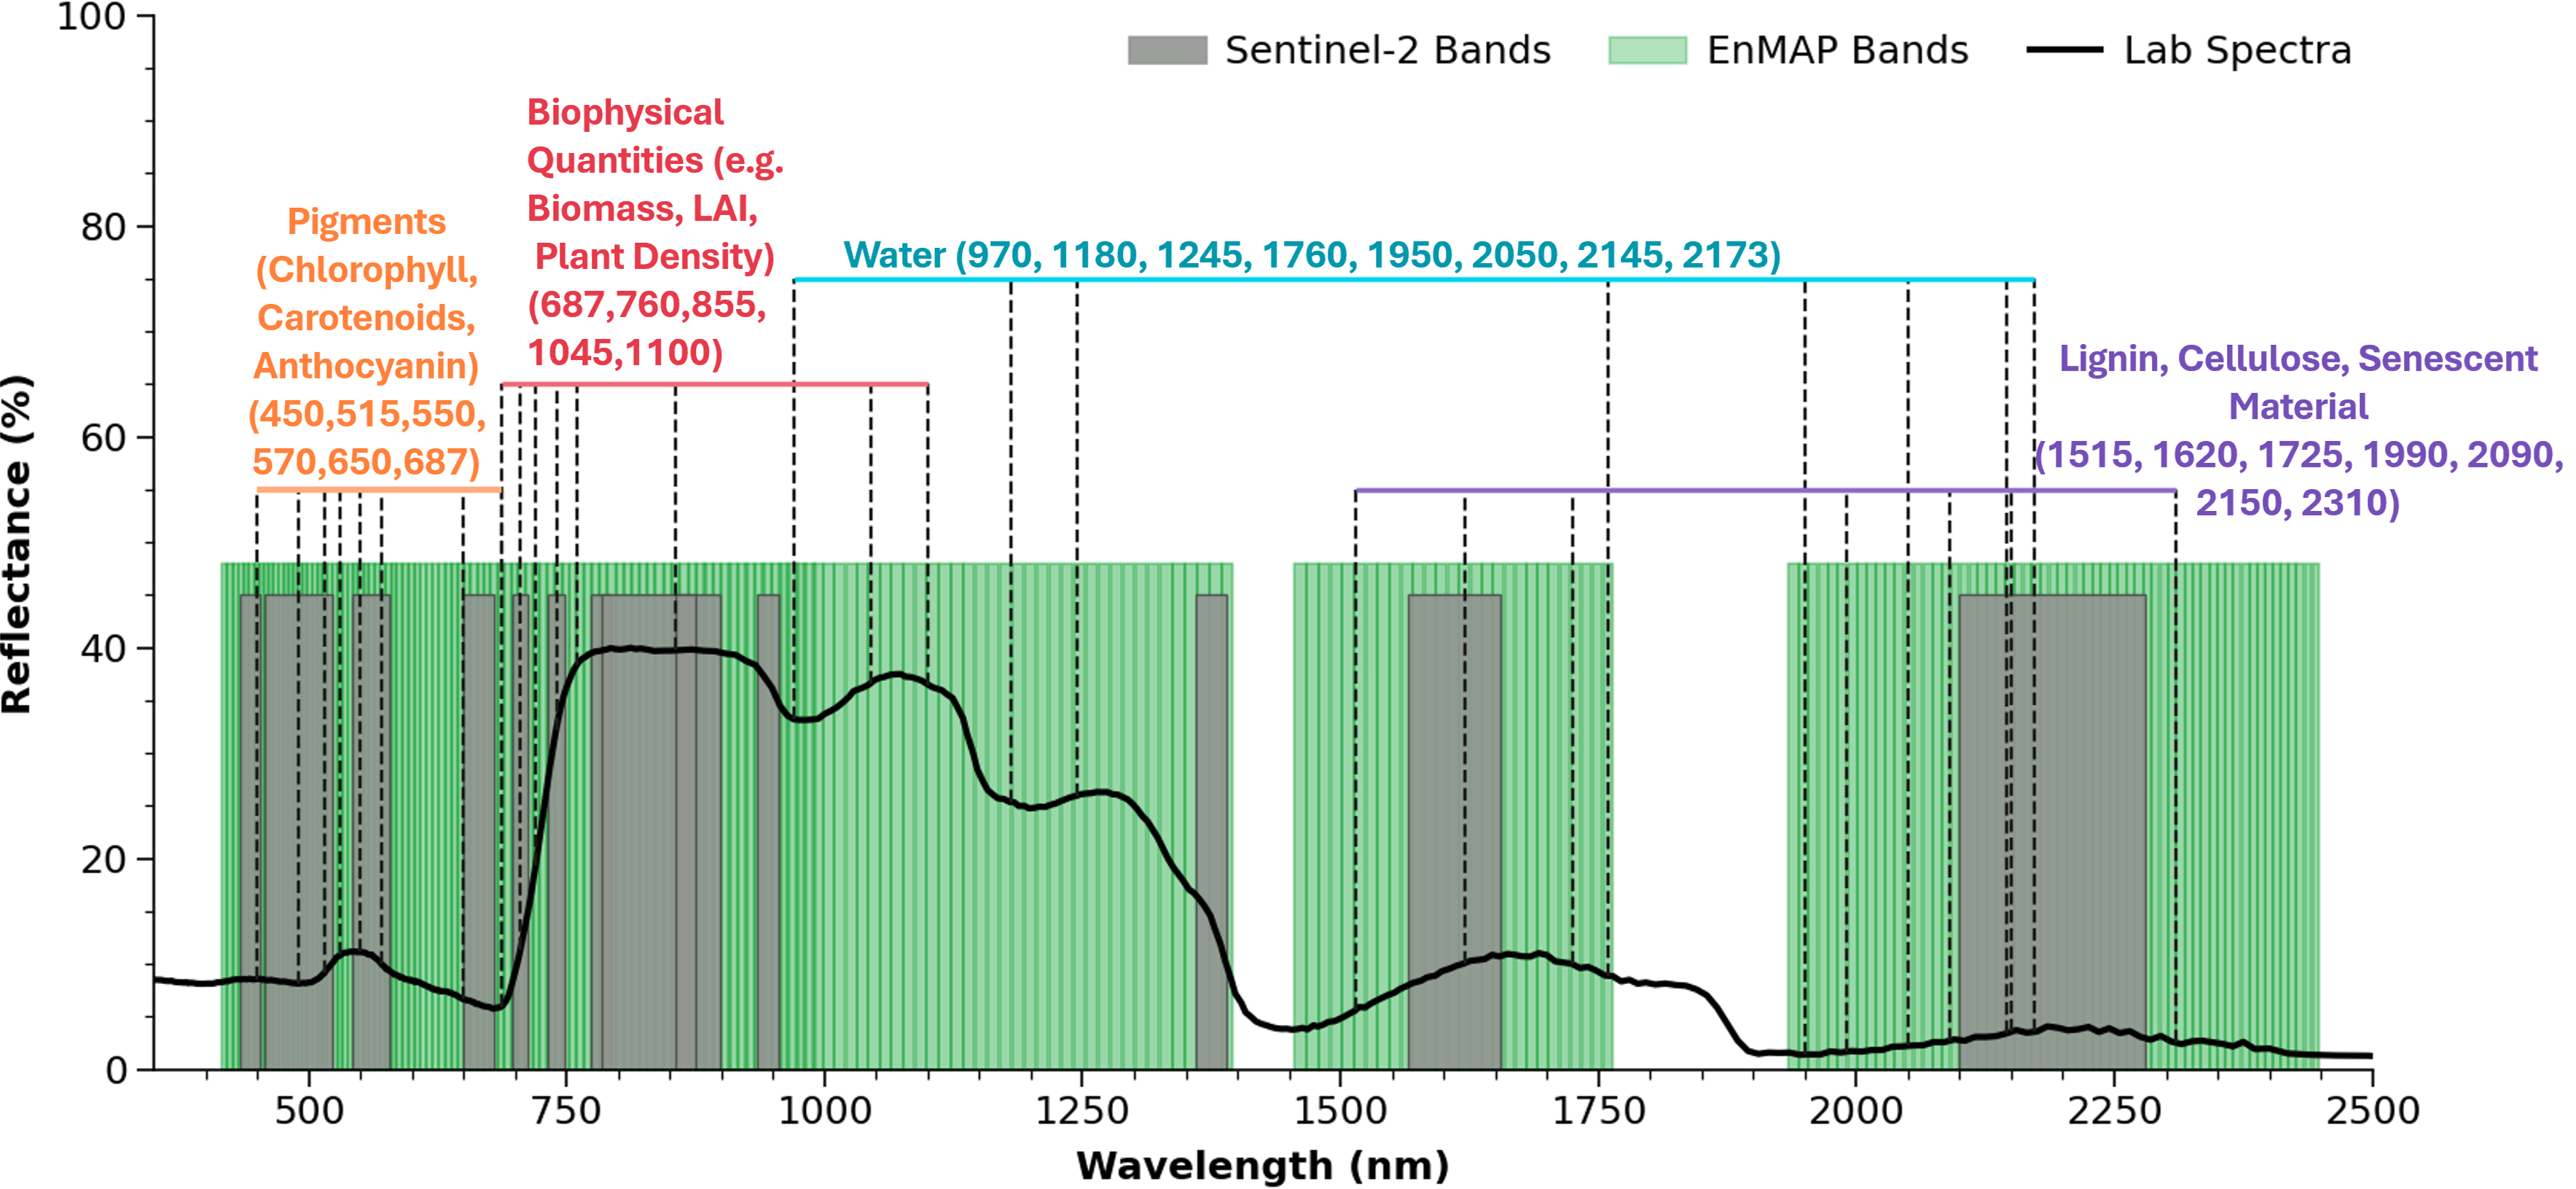
\includegraphics[width=1\textwidth]{figures/fig1_v2.png}
\caption{Vegetation spectra acquired from a laboratory spectrometer alongside the spectral bands of a multispectral sensor (Sentinel-2) and hyperspectral sensor (EnMAP) used in remote sensing. Highlighted are spectral domains sensitive to specific vegetation variables, with absorption features adapted from \citet{thenkabail2013selection,hank2019spaceborne}. }
\label{fig1}
\end{figure}


% missions
In this century, spaceborne hyperspectral missions, including Hyperion (2002)\cite{ungar2003overview}, and recently DESIS (2018)\cite{alonso2019data}, GaoFen-5 (2018)\cite{liu2019advanced}, HISUI (2019)\cite{iwasaki2011hyperspectral}, PRISMA (2019)\cite{loizzo2019prisma}, EnMAP (2022)\cite{guanter2015enmap}, EMIT (2022) \cite{thompson2023orbit} and PACE (2024) \cite{werdell2024life} have gradually enabled global hyperspectral data collection. In addition to the current spaceborne scientific hyperspectral missions, key upcoming operational missions are scheduled for launch after the proposed EcoSpectra project: ESA's Copernicus Hyperspectral Imaging Mission (CHIME), planned for 2028 (CHIME A) and 2030 (CHIME B)\cite{nieke2018towards}, NASA's Surface Biology and Geology (SBG) mission\cite{cawse2021nasa}, set for 2028, and SHALOM\cite{feingersh2015shalom} developed by Italy and Israel. These missions will significantly improve spatial coverage and revisit times, enabling a more detailed and frequent global hyperspectral archive, given that an intercalibration of these sensors is achieved. 

% research gap
Hyperspectral data thus promise great opportunities for quantifying plant traits with upcoming spaceborne missions. However, key challenges remain in realising this potential for effective ecosystem monitoring in concert with established techniques.
First, long-term ecosystem monitoring requires consistent historical data spanning decades, which hyperspectral observations currently lack. Even with new missions underway, the absence of historical coverage hinders long-term analyses of the ecosystem.
Second, assuming this gap is addressed, it has not yet been determined how hyperspectral data can be integrated into existing long-term regional and global monitoring frameworks to maximise its potential and enhance analytical capacity and ecological insight.
This paper tackles the first challenge in Section \ref{sec2} and explores the second in Section \ref{sec3}, offering a path forward for leveraging hyperspectral data in ecosystem monitoring.


\renewcommand{\tabularxcolumn}[1]{>{\raggedright\arraybackslash}p{#1}}
\small
\begin{table}[htbp]
\begin{tabularx}{\textwidth}{
  p{\dimexpr 0.15\textwidth}  % Trait Description
  p{\dimexpr 0.25\textwidth}  % Relevant Process
  p{\dimexpr 0.40\textwidth}  % Ecosystem Process
  p{\dimexpr 0.05\textwidth}  % Retrieval Source
}
\toprule
\textbf{Trait (Abbreviation)} & \textbf{Physiological Process} & \textbf{Ecosystem Process / Climate Relevance} & \textbf{Retrieval Source} \\
\midrule
Chlorophyll content (Chl) & Photosynthesis & Strong proxy for photosynthetic capacity, productivity, and nutrient stress detection. & HS; MS\\
\midrule
Carotenoid content (Car) & Photoprotection, light harvesting & Indicates photoprotection, useful for tracking drought or high-light stress. & HS; MS\\
\midrule
Anthocyanin content (Anth) & Stress response, UV protection & Sensitive to abiotic stress (UV, cold), less directly linked to productivity. & HS; MS \\
\midrule
Nitrogen content (N) & Protein synthesis, photosynthesis & Controls photosynthesis, growth, and is an early indicator of nutrient limitation. & HS\\
\midrule
Phosphorus content (P) & ATP synthesis, nucleic acids & Limits productivity especially in tropical or weathered soils; links to C allocation strategies. & HS\\
\midrule
Potassium content (K) & Osmoregulation, stomatal conductance & Key to osmotic regulation and drought tolerance; affects stomatal conductance. & HS\\
\midrule
Magnesium content (Mg) & Chlorophyll core, enzyme activation & Central to chlorophyll molecule and enzyme function; affects stress sensitivity. & HS\\
\midrule
Sulfur content (S) & Amino acids, redox balance & Indirectly affects protein synthesis and redox regulation; harder to monitor. & HS\\
\midrule
Boron content (B) & Cell wall structure, reproductive development & Important for reproduction and cell wall function; indirect ecosystem effects. & HS\\
\midrule
Copper content (Cu) & Electron transport, redox reactions & Involved in redox reactions, minor influence at ecosystem scale. & HS\\
\midrule
Manganese content (Mn) & Photosystem II activity, redox regulation & Important in photosynthesis and ROS control, but limited large-scale impact. & HS\\
\midrule
Carbon content (C) & Biomass accumulation, respiration & Key trait in leaf economic spectrum; predicts trade-offs in resource use and longevity. & HS \\
\midrule
Calcium content (Ca) & Cell wall stability, signalling, & Used in biomass and stoichiometric modelling; influences decomposition. & HS\\
\midrule
Cellulose content & Cell wall formation, structural support & Structural role in cell walls; not often modelled in ecosystem responses. & HS \\
\midrule
Fibre content & Mechanical support, digestion resistance & Strong predictor of litter decomposition rates and carbon turnover. & HS\\
\midrule
Lignin content & Cell wall rigidity, decomposition resistance & Key to biomass structure and carbon cycling via decomposition. & HS\\
\midrule
Leaf Mass per Area (LMA) & Photosynthetic efficiency, leaf economics & Influences herbivory and digestibility, affects trophic interactions. & HS; MS\\
\midrule
Leaf Area Index (LAI) & Radiation interception, productivity & Directly linked to canopy photosynthesis, water use, and light interception. & HS; MS\\
\midrule
Equivalent Water Thickness (EWT) & Leaf hydration, transpiration & Reflects drought sensitivity, transpiration regulation, and water availability. & HS; MS \\
\midrule
Non-Structural Carbohydrates content (NSC) & Growth, respiration, recovery & Strong predictor of stress resilience, recovery from disturbance, and survival. & HS\\
\bottomrule
\end{tabularx}
\caption{Plant traits can be estimated from hyperspectral (HS) and/or multispectral (MS) data. Their relevance to physiological and ecosystem processes, as well as their remote sensing retrieval sources, are summarised in the following traits list, adapted from the hyperspectral trait retrieval study by Cherif et al. \cite{cherif2023spectra}.}
\label{table1}
\end{table}



\section{Target 1: Build time series with hyperspectral information} \label{sec2}

The benefits of the rich spectral information of hyperspectral data are currently affected by their limited temporal resolution, as the technology is relatively new. The current lack of dense time series has restricted their integration into ecosystem studies, which demand continuous or frequent observations to monitor dynamic processes such as phenology, stress responses, or productivity. The scarcity of temporally dense spaceborne hyperspectral data stems from short historical archives and low revisit frequencies of current hyperspectral sensors, small sensor footprints, and high acquisition costs. Even when some hyperspectral acquisitions are available, the number of time points is typically too sparse for constructing robust time series needed in ecological analyses\cite{lausch2015deriving}.

To address this, we propose using multispectral data with high temporal frequency, such as those from Sentinel-2, to extend the temporal coverage of hyperspectral-derived information. By correlating hyperspectral and multispectral observations at overlapping time points, models can be trained to predict hyperspectral-derived plant traits across more timesteps using multispectral data (see Fig.~\ref{fig2}). 

\begin{figure}[h]
\centering
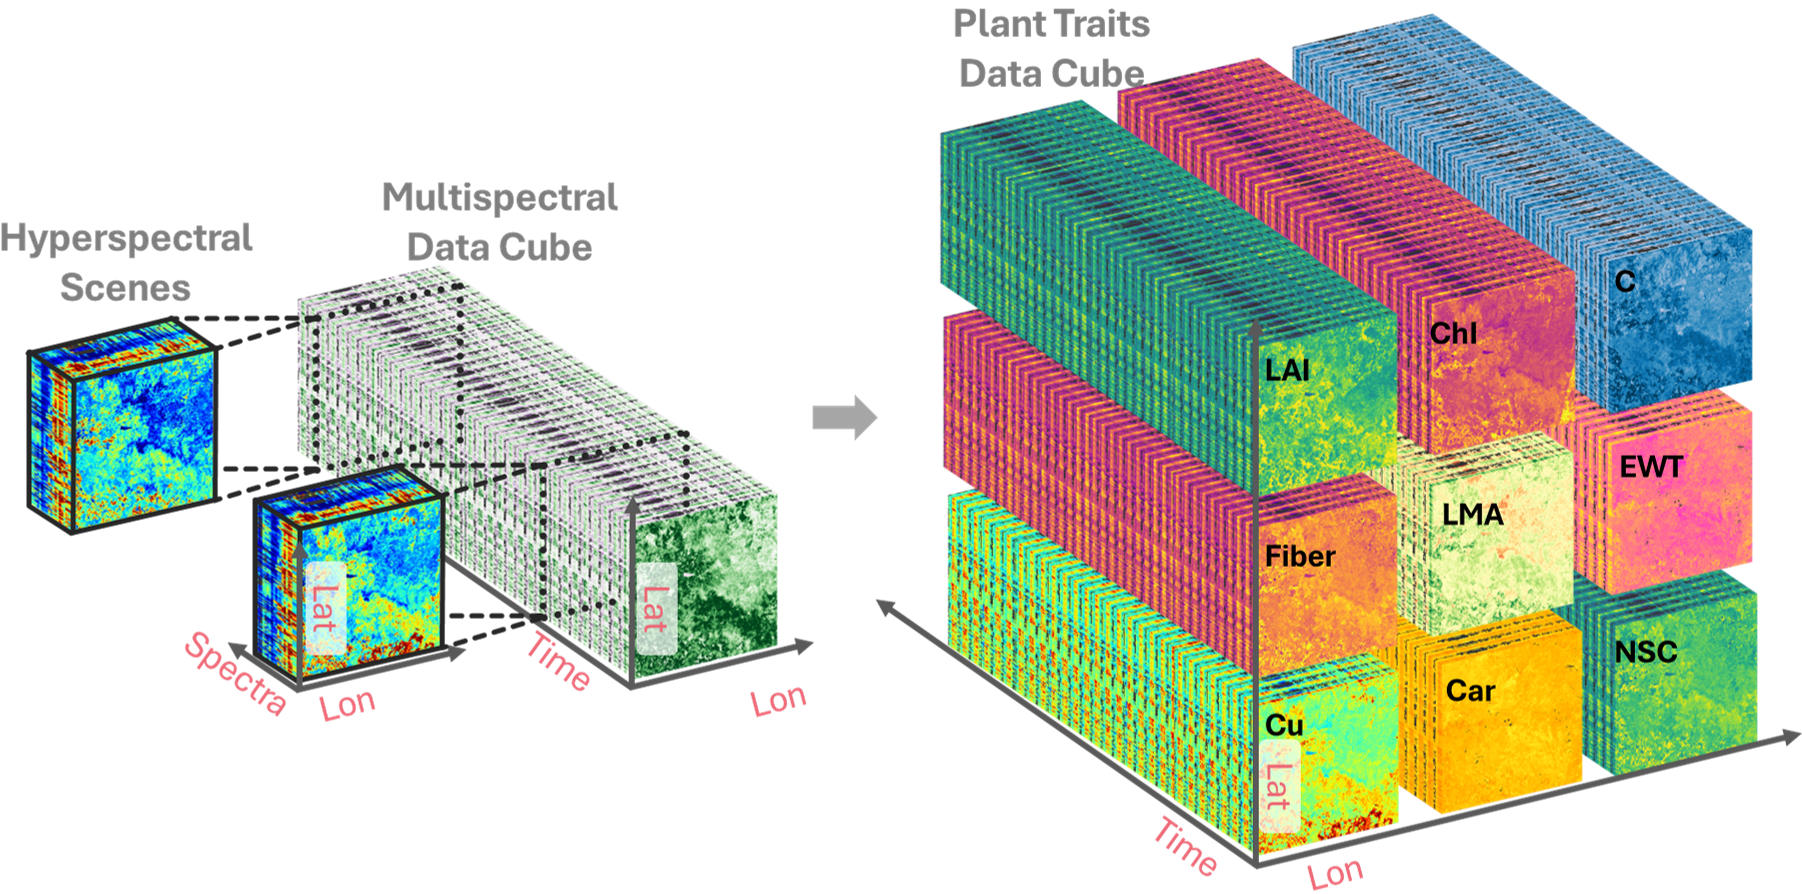
\includegraphics[width=0.85\textwidth]{figures/fig2_v6.png}
\caption{Conceptual illustration of constructing a time series using hyperspectral and multispectral data. On the left, several hyperspectral data cubes (EnMAP; spatial and spectral dimensions) and a time series multispectral data cube (Sentinel-2; spatial and temporal dimensions) are shown. Spectral bands of Sentinel-2 are omitted for clarity. The multispectral data provide a dense temporal baseline, while the hyperspectral data, available at fewer time points, are fused with the multispectral observations. On the right, the resulting plant trait data cube, derived from hyperspectral bands, benefits from the dense and stable temporal coverage provided by the multispectral time series. The demonstration area is the Bavarian Forest National Park. The data cube is visualised using Lexcube \cite{sochting2023lexcube}.}
\label{fig2}
\end{figure}


Notably, in the past two decades, remote sensing and computer vision researchers have developed numerous methods for fusing hyperspectral and multispectral data, primarily to improve the spatial resolution \cite{yokoya2017hyperspectral} of hyperspectral images. These spatial fusion models aim to reconstruct high-spatial-resolution hyperspectral data by exploiting the spectral redundancy between multispectral and hyperspectral imagery. Many of the models, designed initially for spatial fusion, such as sparse representation-based methods, deep learning fusion networks, or hybrid regression frameworks, can be repurposed to enhance temporal resolution. These models are fundamentally based on learning the relationships between multispectral and hyperspectral spectral patterns, and this principle can be extended to temporal interpolation. The survey of these methods, though not exhaustive here, can be grouped into four main categories. Model-based approaches include traditional dimensionality reduction techniques (e.g., Intensity-Hue-Saturation (IHS) transformation, Principal Component Analysis (PCA)), multiresolution analysis methods (e.g., wavelet, contourlet), and subspace-based models such as Coupled Nonnegative Matrix Factorization (CNMF) \cite{yokoya2017hyperspectral}. Sparse representation-based methods encompass joint sparse representation, convolutional sparse coding, and spatial-spectral sparse representation techniques \cite{xing2022fusion,dian2019multispectral}. Deep learning-based approaches cover a broad spectrum of architectures, including Convolutional Neural Networks (CNNs), autoencoders, Generative Adversarial Networks (GANs), transformers, hybrid CNN-transformer models, and attention-enhanced frameworks \cite{khader2022model,gao2023enhanced,jia2023multiscale,hong2021interpretable}. These methods can be used to correlate hyperspectral and multispectral data and leverage multispectral observations to estimate missing hyperspectral information at unobserved timesteps within the same study area. However, reconstructing the full hyperspectral signal as an intermediate step prior to plant trait estimation can be computationally inefficient and prone to compounded uncertainty, first during spectral reconstruction, and then again during trait estimation from the reconstructed hyperspectral signal.

% To overcome these limitations, foundation models have emerged that bypass explicit spectral reconstruction by learning task-relevant representations directly from multi-modal inputs. Among these foundation models, transformer-based architectures have shown promise for handling pixel-level time series from multi-modal data. One illustrative example is the Pretrained Remote Sensing Transformer (Presto) \cite{tseng2023lightweight}, which aligns closely with our proposed approach of using temporally dense multi-spectral data. Presto learns temporal representations from multi-modal time series data (e.g., Sentinel-1, Sentinel-2), combined with auxiliary metadata such as topography and climate variables. It employs a masked autoencoding strategy to learn informative temporal embeddings by reconstructing missing spectral bands or timesteps. This approach is computationally efficient and flexible, allowing the same pretrained model to support a range of downstream tasks, including crop type classification, land cover mapping, and algal bloom prediction. Although this approach has not yet been applied to plant trait prediction, its architecture is well-suited for this purpose. Moreover, the framework can be extended to flexibly accommodate hyperspectral data by enabling the model to ingest a broader and variable number of spectral bands, so that when hyperspectral observations are available, they can directly enrich the input representation and improve trait prediction.

To overcome these limitations, multi-modal models can bypass spectral reconstruction by learning task-relevant representations directly from different sources (also known as different modalities). Among these models, transformer-based architectures have shown promise for handling pixel-level time series from multi-modal data. From here, there are two pathways to follow: a classical supervised approach with annotated data, or a self-supervised approach to pre-train the model with unlabelled data. While the first case is straightforward, collecting the required data can be expensive and availability is limited, delivering overfitted models due to few samples used in training. In the second case, while there is no need for labeled data, the resources needed to pretrain a model on a large dataset that is able to capture an accurate representation of Earth processes can be enormous. However, the second case brings the opportunity to fine-tune the model for different downstream tasks, such as crop type classification, land cover mapping, or algal bloom prediction. One illustrative example is the Pretrained Remote Sensing Transformer (Presto) \cite{tseng2023lightweight}, which aligns closely with our proposed approach of using temporally dense multi-spectral data. Presto learns temporal representations from multi-modal time series data (e.g., Sentinel-1, Sentinel-2), combined with auxiliary metadata such as topography and climate variables. It employs a masked autoencoding strategy to learn informative temporal embeddings by reconstructing missing spectral bands or timesteps. Although this approach has not yet been applied to plant trait prediction, its architecture is well-suited for this purpose. Moreover, the framework can be extended to flexibly accommodate hyperspectral data by enabling the model to ingest a broader and variable number of spectral bands, so that when hyperspectral observations are available, they can directly enrich the input representation and improve trait prediction.


To avoid the computational and data management burden of modelling hundreds of spectral bands across time, we furthermore recommend using hyperspectral observations to first retrieve key plant traits (e.g., chlorophyll content, leaf area index, leaf dry matter) \cite{cherif2023spectra}. These traits can then be modelled over time using multispectral time series data, significantly reducing data dimensionality and enhancing ecological interpretability.

% uncertainty control
Retrieving plant traits from hyperspectral data typically involves three core steps: (1) spectral preprocessing and correction (e.g., atmospheric correction, noise filtering), (2) transformation or feature extraction (e.g., vegetation indices, spectral derivatives, radiative transfer inversion), and (3) model-based trait estimation. Trait estimation is commonly implemented using statistical regressions (e.g., PLSR), physical model inversion (e.g., PROSAIL), or machine learning approaches (e.g., random forest, CNNs) trained on reference trait datasets \citep{Blackburn2007, LeMaire2004, Cherif2023}. Model calibration relies on trait reference data collected from \textit{in situ} or laboratory measurements (e.g., leaf chlorophyll content, LMA, nitrogen). To ensure generalizability, calibration is ideally conducted using a representative, diverse training dataset covering the range of canopy structures, species, and environmental conditions relevant to the study area \citep{Verrelst2015, Kattenborn2019}. Validation of hyperspectral-derived traits is typically done using an independent set of trait observations not included in the calibration. Statistical metrics such as R$^2$, RMSE, and bias are used to assess model performance. When repeated \textit{in situ} or laboratory data are not available, cross-validation or transfer learning methods may be used to estimate uncertainty across space or time. Major sources of uncertainty include sensor noise, variability in viewing geometry, imperfect atmospheric correction, and mismatch in spatial scale between hyperspectral imagery and field plots \citep{Schweiger2020, Mederer2025}. To mitigate these uncertainties, recent work has explored hybrid models that combine radiative transfer simulations with empirical machine learning, or use physics-informed neural networks to constrain trait predictions with ecological realism \citep{Sun2024, She2024}. As a best practice, we recommend reporting uncertainty estimates (e.g., prediction intervals, ensemble spread) alongside trait predictions and validating results across multiple sites and time periods where possible.

\section{Target 2: Explore the full potential of hyperspectral data} \label{sec3}

As plant trait time series become increasingly accessible through hyperspectral–multispectral fusion, their integration into ecological analysis opens new avenues beyond traditional vegetation indices based on multispectral data. These trait-based data cubes—comprising key variables such as chlorophyll content, leaf mass per area (LMA), equivalent water thickness (EWT), and leaf area index (LAI)—offer high-resolution, biochemically grounded information that supports a more mechanistic understanding of ecosystem function and resilience. In this section, we outline three major pathways through which these hyperspectral-derived trait cubes can support ecosystem monitoring: (1) integration with complementary data sources to enrich existing monitoring products; (2) support for ecological and Earth system model development; and (3) enhanced global change research through trait-based indicators.


\subsection{Integrating Complementary Data Sources and Enriching Monitoring Products}\label{subsec1}

% SIF
% environmental DNA, below ground diversity?
Integrating hyperspectral remote sensing with other Earth observation and \textit{in situ} measurements is essential for advancing ecological monitoring, improving trait estimation, and supporting model validation. Hyperspectral sensors provide detailed spectral information linked to plant biochemical and physiological traits, but their effectiveness increases when combined with complementary data sources that capture structural and functional ecosystem properties. For example, coupling hyperspectral data with canopy structure from LiDAR or SAR improves trait characterisation in vertically complex forests. Likewise, integrating hyperspectral and thermal data enables more accurate detection of plant stress and assessments of functional diversity under climate extremes. It further offers the opportunity to identify the actual stressor through investigating the degradation of specific traits such as leaf water content, pigments or nitrogen status. Such multi-source datasets enhance the robustness of trait retrievals and serve as intermediate validation layers. Validation is the bottleneck when ensuring the reliability of hyperspectral products \citep{cherif2023spectra,mederer2025plant}, and \textit{in situ} observations, such as those from eddy covariance systems, provide essential flux data for calibration and evaluation. The FLUXNET network, with over 140 globally distributed sites across diverse biomes, offers standardised, high-quality localised remote sensing measurements that anchor remote observations and inform ecosystem models. Together, these integrated approaches establish a robust framework for generating and validating remote sensing products in ecological research.

%genetic diversity
Plant traits derived from hyperspectral data can serve as functional proxies for genetic diversity, particularly when these traits reflect phenotypic variation regulated by heritable genetic factors \citep{Violle2007, Funk2017, Zhao2021}. Many plant traits observable via hyperspectral sensors—such as chlorophyll content, leaf mass per area (LMA), and pigment composition—exhibit intraspecific variation shaped by the interactions of genotypes with their environment \citep{Asner2015, Schweiger2018}. Genetic diversity—defined as genomic variation within and between populations—is a foundation of phenotypic plasticity, adaptive potential, and ecosystem resilience \citep{Barrett2008, Jump2009}. In forest ecosystems, where long-lived species dominate and shape community structure, genetic variation underpins environmentally contingent variation in growth, phenology, and stress tolerance \citep{Petit2006, Alfaro2014}. While molecular methods remain the gold standard for assessing genetic diversity, remotely sensed trait diversity offers a scalable and ecologically meaningful proxy. It has been shown to correlate with genetic structure in some systems and holds promise for scaling genetic information to the landscape level (recently reviewed in \cite{cavender2025spectral}. Moreover, phenotypic variability observed across populations—such as trait differences under drought or nutrient stress—can reflect genotype–environment interactions and local adaptation, and enable analyses of the resistance and resilience of communities to stress \citep{Shakoor2017, Bai2023}. Global policy frameworks increasingly recognise trait diversity and population-level indicators as useful surrogates for monitoring genetic diversity, particularly in large-scale or data-limited contexts \citep{Hoban2020, Hoban2024}.


\subsection{Supporting the Development of Ecological and Earth System Models}\label{subsec3}

Ecological and Earth system models are critical for predicting carbon dynamics, vegetation-climate interactions, and ecosystem responses to disturbance. However, a major limitation across model classes lies in their reliance on static, generalised plant trait inputs and infrequent land surface updates. These assumptions fail to represent transient ecosystem states and trait plasticity, leading to considerable uncertainty under changing environmental conditions (and links to genotype-by-environment interactions). Integrating trait cubes—biweekly, spatially continuous time series of plant functional traits derived from hyperspectral observations—offers a new path toward improving model structure, parameterisation, and scaling.



% + radiative transfer models
Radiative transfer models (RTMs) such as PROSAIL \cite{jacquemoud2009prospect+} and DART \cite{gastellu2004dart} provide a physically grounded framework to simulate trait values from canopy reflectance.
. Integrating time series or plant traits retrieved from hyperspectral data enhances the realism of RTM inversions, improving alignment with seasonal and phenological dynamics \cite{verrelst2019quantifying,mederer2025plant}. However, most RTMs oversimplify real-world vegetation by assuming fixed canopy structures, homogeneous leaf distributions, and static physiology. As a result, they often fail to reproduce observed spectra in heterogeneous or stress-responsive ecosystems (ill-posed problem) \cite{kattenborn2019radiative,ali2021machine}. Despite these limitations, RTMs remain valuable—particularly in data-scarce regions and as physical priors in hybrid modeling approaches. Embedding RTMs into neural networks as differentiable components allows models to retain physical interpretability while adapting to observational data \cite{sun5107112bridging,she2024spectra}. Transfer learning extends their utility by using RTM simulations for pre-training, followed by fine-tuning on field data \cite{zhang2021domain}. Together, these strategies bridge physical modelling and data-driven learning, improving generalisation and trait estimation in diverse ecosystems.


% Individual-Based and Gap Models
Individual-based models (IBMs) such as FORMIND \cite{kohler1998effects} and FORMIX3 \cite{huth1998rain} explicitly simulate forest structure, competition, and succession by modeling trees as discrete units. These models capture stand dynamics well but typically rely on static or coarsely aggregated trait inputs (e.g., fixed leaf mass per area or chlorophyll content), and land cover inputs are updated annually or remain fixed. As a result, IBMs struggle to represent seasonal transitions, physiological responses, or disturbance legacies, reducing their accuracy in simulating mortality, recruitment, and biomass turnover. Traits cubes derived from hyperspectral time series enable the introduction of spatially and temporally dynamic trait inputs—such as seasonal variation in chlorophyll, EWT, or LMA—thereby improving predictions of individual tree growth, stress response, and regeneration. This supports better representation of competitive interactions, phenological synchrony, and stand-scale heterogeneity.

% Dynamic Global Vegetation Models (DGVMs)
Ecosystem process models such as LPJ and Biome-BGC represent vegetation at large scales using fixed plant functional types (PFTs), each assigned with mean trait values. This approach oversimplifies functional diversity and ignores intra- and inter-annual variation in key traits such as nitrogen concentration, LAI, or non-structural carbohydrates (NSC) \cite{verrelst2019quantifying,mederer2025plant}. Land surface properties are also assumed to be temporally stable over simulation intervals, which limits model responsiveness to droughts, land-use changes, or disturbance events. Incorporating time-series trait data into DGVMs enables the transition from coarse PFT-based parameterizations to trait-based dynamic modeling. This improves the physiological realism of carbon and water flux simulations and increases predictive skill under extreme climate events or changing vegetation regimes. For example, real-time NSC and EWT dynamics can inform ecosystem vulnerability and carbon allocation strategies under stress.

% Eco-Physiological Submodels
Many ecosystem models contain embedded physiological components such as the Farquhar photosynthesis model or the Ball–Berry stomatal conductance model, which require accurate inputs of traits including Vcmax, Jmax, chlorophyll content, and LMA \cite{sun5107112bridging,ali2021machine}. However, in practice, these submodels are typically run with trait values that are either constant or calibrated under limited conditions, failing to reflect phenological shifts or physiological acclimation. By providing frequent, spatially resolved trait updates, traits cubes enhance the mechanistic representation of photosynthetic efficiency, light-use dynamics, and stress physiology. %Integrating seasonally varying chlorophyll and LMA directly informs models of GPP and respiration, while time-varying NSC and EWT support estimation of drought-induced mortality risk. Embedding these trait updates improves the fidelity of ecosystem carbon cycle predictions, especially under transient or disturbed conditions.



\subsection{Enhancing Global Change Research with Trait Cubes}\label{subsec4}
Despite progress in Earth observation and ecosystem modeling, significant limitations remain in understanding vegetation responses to global change across spatial scales \cite{higgins2023shifts}. Most global vegetation products—particularly those derived from climate-driven dynamic global vegetation models (DGVMs) or coarse-resolution satellite data—are simplified representations that fail to capture plant functional diversity and physiological traits at fine spatial and temporal scales. Downscaled datasets often rely heavily on climate variables and land cover classifications, introducing structural uncertainty and masking sub-grid ecological heterogeneity. In contrast, hyperspectral trait cubes provide rich, high-resolution spatiotemporal data on ecophysiological traits, such as chlorophyll content, LMA, or equivalent water thickness, offering new opportunities to monitor ecosystem changes with greater specificity and accuracy \cite{zhao2021hyperspectral}. These data can help reduce uncertainty in ecosystem assessments by grounding predictions in empirically observable traits rather than generalized proxies or model assumptions.

Plant traits offer a mechanistic link between organisms and their environment, representing functional strategies for survival, growth, and resource use under changing conditions \cite{solbrig1994plant,funk2017revisiting}. Incorporating trait-based data into global change research thus enhances the capacity to assess not only what is changing but how and why it changes \cite{xu2021trait,green2022trait}. Trait cubes allow for continuous tracking of functional diversity and vegetation health across time and space, enabling a shift from static land cover maps to dynamic, physiology-informed monitoring. Moreover, such data enable trait-based indicators of ecosystem vulnerability, resilience, and tipping points—key aspects often missed in purely spectral or structural products \cite{gallagher2021guide,brown2023trait}.

This trait-based lens is particularly important for understanding and predicting the stability of terrestrial carbon sinks \cite{xu2021trait}. Accurate trait data can inform assessments of photosynthetic capacity, water-use efficiency, and stress responses—critical for modeling carbon sequestration potential and its directionality under climate change \cite{gago2014opportunities}. Integrating trait cubes into Earth system models could therefore improve forecasts of terrestrial carbon fluxes by linking biological processes with climate variability and disturbance regimes \cite{anderegg2015tree,peng2021global}. Additionally, trait data can reveal spatial patterns of vegetation adaptation and maladaptation, offering early-warning signals of biome shifts, forest dieback, or ecosystem transitions that traditional land cover maps may miss \cite{scheffer2009early,boulton2022pronounced,tai2023linking}. These insights are vital for designing effective mitigation and adaptation strategies in the Anthropocene.




\section{Challenges and opportunities}\label{subsec2}
Achieving these targets requires integrating traditional methods with emerging technologies, interdisciplinary collaboration, and open science initiatives.

% challenges--
% uncertainty
Key challenges in integrating hyperspectral data into ecological monitoring include overcoming data availability and temporal coverage constraints, computational and technical hurdles, and fostering interdisciplinary collaboration. Despite the promise of more spaceborne hyperspectral sensors, such as CHIME and SBG in the coming decade, current sensors like EnMAP and PRISMA offer limited spatial and temporal coverage. Although future missions may expand coverage, they cannot address the lack of historical data, necessitating the reconstruction of past data using other sources—an approach that inherently introduces uncertainty. Furthermore, maintaining consistency in techniques and sensor settings during ecosystem monitoring is essential to ensure robust long-term statistical analyses. This requirement must be carefully balanced with integrating new technologies.

% computational and expert knowledge required
The computational and technical complexities of hyperspectral data processing are also substantial. For instance, even a modest study area of 30 km by 30 km, sampled bi-weekly over a decade, can result in XX terabytes of data, posing storage, processing, and analysis challenges. Additionally, effective use of hyperspectral data demands not only advanced machine learning models for data fusion (e.g., hyperspectral, multispectral, LiDAR, SAR) but also scientists with cross-disciplinary expertise who can fully leverage the strengths of each data source. 

% the constantly asked question: extensive data
For hyperspectral data, the large volume of information remains a persistent challenge. One major limitation is the constrained satellite-to-ground data downlink capacity, which complicates data acquisition. To address this, missions such as EnMAP and PRISMA adopt a task-based acquisition strategy. When a specific area is targeted for observation, neighbouring regions are often deprioritised or omitted entirely, resulting in incomplete data coverage. To mitigate these limitations, edge computing has gained significant attention over the past decade. This approach is particularly favoured by small commercial hyperspectral satellite missions, as it allows for onboard data processing, reducing the need for extensive downlink and enabling more efficient use of limited transmission bandwidth. For ecological applications, it is recommended that users directly utilise plant trait products derived from hyperspectral data, such as the example presented in Section \ref{sec2}, or apply simplified computational models to process long-term hyperspectral datasets. As data volumes continue to grow and machine learning models evolve rapidly, technological advancements are expected to further alleviate the challenges associated with hyperspectral data acquisition and processing.


% call for scientist
Here, we make a call to action for researchers and policymakers. Effective cross-disciplinary collaboration is essential for bridging the gaps between remote sensing and ecology, ensuring a seamless connection between data producers and end-users, and fostering a positive feedback loop that enhances data product quality. To fully realise the potential of global hyperspectral data applications, it is crucial to promote the scalable collection and integration of hyperspectral data from field, UAV, and airborne platforms. These datasets should be openly shared and adhere to standardised protocols, ideally established by leading laboratories, to ensure consistent data pre-processing and sharing practices. Policymakers who understand the capabilities of hyperspectral data—particularly its ability to detect detailed ecological traits—will be better equipped to support its integration into ecosystem monitoring and conservation strategies. Such awareness can accelerate the adoption of hyperspectral technology, driving more effective ecological management and climate resilience efforts.



\section{Conclusion}\label{subsec5}

Hyperspectral data enable the quantification of plant and canopy biochemical traits, offering unprecedented insights into ecosystem function. In this paper, we introduce the concept of constructing time series of hyperspectral-derived plant traits already at present, despite limitations on available time series, by leveraging time series of multispectral data. This approach addresses the current limitations in observation frequency that hinder the application of hyperspectral data in real-world ecosystem analyses. We highlight the value of hyperspectral data not only as a standalone resource but also as a complementary input to other datasets, physical models, and biological systems monitoring, enhancing the accuracy and scope of ecological assessments. While we discuss associated challenges—such as data volumes, downlink constraints, interpretability, and processing complexity—we also emphasise emerging opportunities, including edge computing and simplified trait-based analysis approaches. Realising the full potential of hyperspectral remote sensing requires a coordinated global effort to establish priorities and synthesise evidence, including through ecological monitoring networks, open data sharing, and transdisciplinary collaboration among ecologists, remote sensing scientists, data analysts, and policymakers. Looking ahead, we join the call to the ecological community to proactively adopt these advanced technologies to address critical challenges in ecosystem analysis, particularly under accelerating climate change \cite{cavender2025spectral}. Such advancements have the potential to directly inform global ecological governance, providing essential data for conservation planning and evidence-based policy-making.

%%%%%%%%%%%%%%%%%%%%%%%%%%%%%%%


\bmhead{Supplementary information}

If your article has accompanying supplementary file/s please state so here. 

Authors reporting data from electrophoretic gels and blots should supply the full unprocessed scans for key as part of their Supplementary information. This may be requested by the editorial team/s if it is missing.

Please refer to Journal-level guidance for any specific requirements.

\bmhead{Acknowledgements}

We thank Maximilian Soechting for his professional input and constructive suggestions that contributed to the development of Figure 2.

\section*{Declarations}

Some journals require declarations to be submitted in a standardised format. Please check the Instructions for Authors of the journal to which you are submitting to see if you need to complete this section. If yes, your manuscript must contain the following sections under the heading `Declarations':

\begin{itemize}
\item Funding


We want to thank the editors and anonymous reviewers for their constructive comments that helped to improve the manuscript. The authors acknowledge the support from the German Federal Ministry for Economic Affairs and Climate Action (BMWK) and the German Aerospace Center (DLR) for the project "TEE Cube - Time-varying AI-based Mapping of Ecosystem Conditions and Extents Using Multi-source Earth Observation Data Cubes".

\item Conflict of interest/Competing interests (check journal-specific guidelines for which heading to use)
\item Ethics approval and consent to participate
\item Consent for publication
\item Data availability 

The authors acknowledge the German Aerospace Center (DLR) for sharing airborne flight campaign data.


\item Materials availability
\item Code availability 
\item Author contribution
\end{itemize}

\noindent


\begin{appendices}
\section{}\label{secA1}
\end{appendices}


\bibliography{bibliography}% common bib file
%% if required, the content of .bbl file can be included here once bbl is generated
%%\input sn-article.bbl

\end{document}
